\documentclass[12pt]{article}
\usepackage[margin=0.3in,top=0.25in,bottom=0.4in]{geometry}
\makeatletter
\renewcommand{\@maketitle}{\newpage\null\vskip -3.5em\begin{center}{\LARGE \@title \par}\end{center}\par\vskip 0.2em}
\makeatother
\usepackage{amsmath,amssymb}
\usepackage{booktabs}
\usepackage{graphicx}
\usepackage{hyperref}
\setlength{\parskip}{0.6em}
\setlength{\parindent}{0pt}
\newcommand{\xpo}{x_{\mathbb{P}}}

\title{The cut on $K_\perp$ and the quark DTMD}
\author{}
\date{}

\begin{document}
\maketitle

\section*{In short}

Paul's comment on the draft: how sensitive is the diffractive (TMD) result to the upper limit
$K_\perp\leq p_\perp$, and is $p_\perp\gg Q_s$ satisfied? Findings (charm quark at fixed $q^+=2p^+$,
proton and Pb at $b_d=0$, $y=0$ and $2$):
\begin{enumerate}
\item With $K_\perp\leq c\,p_\perp$ the result depends strongly on $c$ below $p_\perp\approx3\,Q_{s,A}$
  (factors 2--80), and is stable (few \%) above it. $p_\perp\gg Q_s$ fails in the lowest bins.
\item But $p_\perp$ is not the hard scale of the gluon DTMD: Ref.~[3] (arXiv:2606.04169) requires
  $M_h^2=m_T^2/(z(1-z))\gg Q_s^2$, and the correlation-limit expansion is in $K_\perp$ against $m_T$.
  With $K_\perp\leq c\,m_T$ the result converges: for the proton and for $p_\perp\gtrsim3$~GeV within
  a few \%, for Pb at $p_\perp\lesssim2$~GeV within 10--25\%.
\item The quark DTMD (Sec.~4 of Ref.~[3]; see the note \texttt{quark\_dtmd}) is a valid TMD contribution
  only for $p_\perp\gtrsim5$~GeV, where it is 0.6--1.6\% of the gluon DTMD. It is now included for
  $p_c\geq5$~GeV.
\item With the cut on $m_T$, the diffractive part at $p_\perp\lesssim1$~GeV grows by a factor 2--20,
  so the exclusive part may no longer dominate the lowest $p_{D\perp}$ bins.
\end{enumerate}

\section*{1. Saturation scale and $p_\perp\gg Q_s$}

$Q_s^2=2/r_s^2$ with $\mathcal{N}(r_s)=1-e^{-1/2}$ (fundamental, from
\texttt{AmplitudeLib::}\allowbreak\texttt{SaturationScale}) or $\mathcal{N}_A(r_s)=1-e^{-1/2}$ (adjoint, $\mathcal{N}_A=2\mathcal{N}-\mathcal{N}^2$, which enters the
gluon DTMD); program \texttt{saturation\_scale}, figure \texttt{plots/saturation\_scale.pdf}.
For given $p_\perp$ and $y$, $x<1$ gives $\xpo\geq M_{q\bar q}^2/W^2=m_T^2/(\bar z\sqrt2\,p^+\sqrt{s})$, whose
minimum over the photon energy is $\xpo^{\min}\approx m_Te^{-y}/\sqrt{s}$ ($z\to0$, at $z_h=1$). $Q_s$
decreases with $\xpo$, so $Q_s(\xpo^{\min})$ is the largest relevant value at any photon energy. (The note
\texttt{correlation\_limit} fixes $z=\tfrac12$ instead, with $\xpo^{\min}$ twice as large, and $y=0$--3;
its $Q_s$ are $\approx10\%$ lower at the same $y$.)
\begin{center}
\begin{tabular}{lcccc}
\toprule
 & $Q_{s,A}$, $y=0$ & $Q_{s,A}$, $y=2$ & $p_\perp=Q_{s,A}$ at & $p_\perp=Q_{s,F}$ at \\
\midrule
proton     & 1.05 GeV & 1.38 GeV & 0.8--1.3 GeV & 0.5--0.8 GeV \\
Pb, $b_d=0$ & 1.91 GeV & 2.45 GeV & 1.5--2.3 GeV & 1.0--1.5 GeV \\
\bottomrule
\end{tabular}
\end{center}
($p_\perp$ ranges for $y=-2$ to $2$.) $Q_s$ depends little on $b_d$ in the core of the nucleus
($\approx5\%$ up to $b_d=10$~fm).

\begin{center}
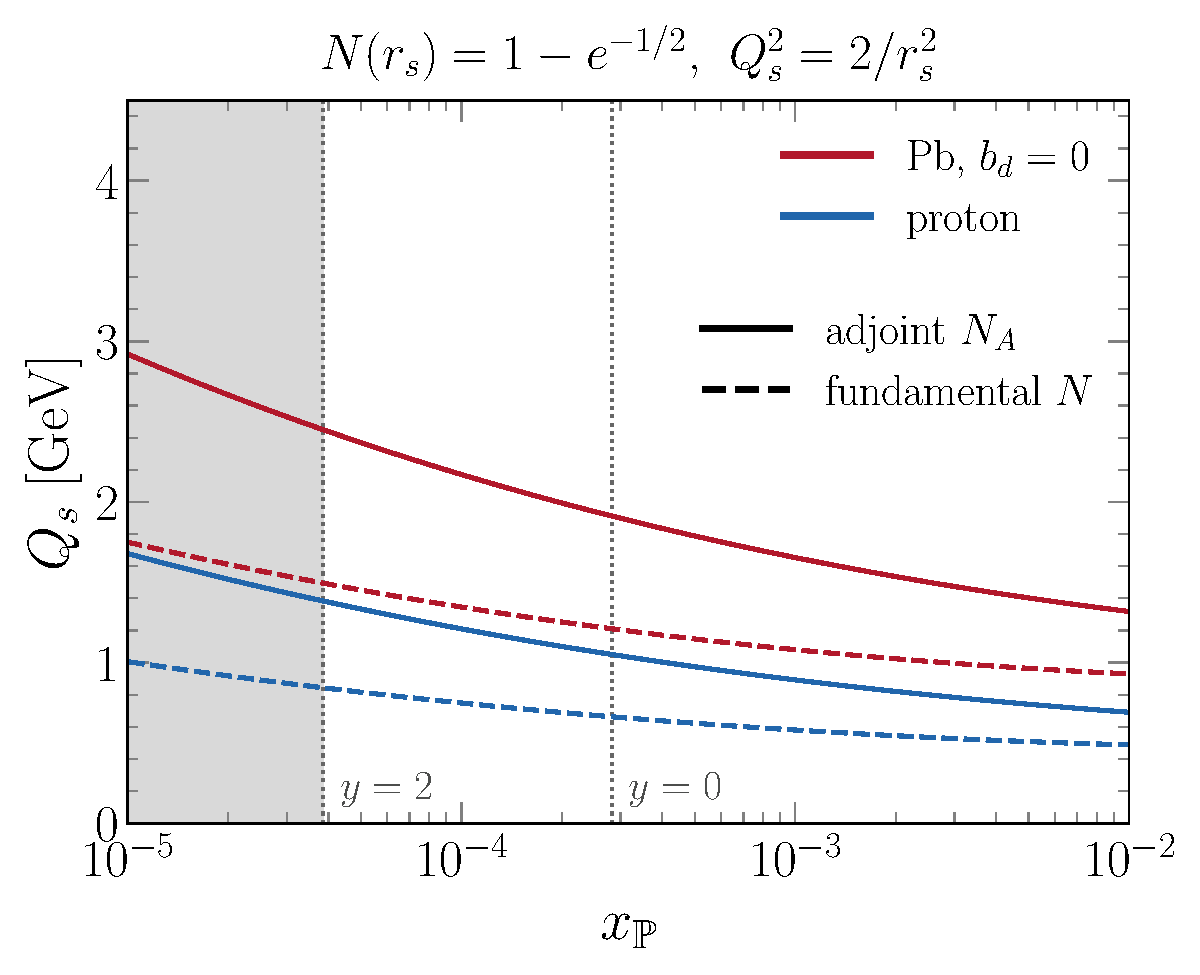
\includegraphics[width=0.48\textwidth]{../plots/saturation_scale.pdf}
\end{center}

\section*{2. The cut $K_\perp\leq c\,p_\perp$}

Gluon DTMD, divided by the result at $c=1$ (VEGAS noise $<1\%$):
\begin{center}
\begin{tabular}{c|cccc|cccc}
\toprule
 & \multicolumn{4}{c|}{proton, $y=0$} & \multicolumn{4}{c}{Pb, $y=2$} \\
$p_\perp$ [GeV] & $c=\tfrac12$ & $c=2$ & $c=4$ & no cut & $c=\tfrac12$ & $c=2$ & $c=4$ & no cut \\
\midrule
0.20 & 0.25 & 3.5  & 9.5  & 19   & 0.24 & 3.9  & 14   & 84   \\
0.84 & 0.39 & 1.58 & 1.82 & 1.95 & 0.29 & 2.6  & 4.2  & 5.6  \\
2.17 & 0.75 & 1.09 & 1.12 & 1.12 & 0.46 & 1.39 & 1.54 & 1.67 \\
3.49 & 0.89 & 1.04 & 1.04 & 1.05 & 0.65 & 1.16 & 1.22 & 1.26 \\
5.61 & 0.96 & 1.01 & 1.02 & 1.02 & 0.83 & 1.06 & 1.09 & 1.10 \\
9.04 & 0.98 & 1.01 & 1.01 & 1.01 & 0.92 & 1.02 & 1.03 & 1.04 \\
\bottomrule
\end{tabular}
\end{center}
Removing the cut changes the result by $<10\%$ for $p_\perp\gtrsim3\,Q_{s,A}$ ($\approx3.5$~GeV proton,
$\approx6$~GeV Pb), as Paul expected. Below $p_\perp\approx Q_{s,A}$ the result is set by the cut. The
curves are nearly universal in $p_\perp/Q_s$.

\section*{3. The hard scale of the gluon DTMD is $M_h$}

Ref.~[3], Eq.~(3.1): the dijet is hard if $M_h^2=Q^2+(P_\perp^2+m^2)/(z_1z_2)\gg Q_s^2$; at $Q^2=0$,
$M_h^2=m_T^2/(z(1-z))\geq4m_T^2$. The correlation-limit expansion, Eqs.~(3.16)--(3.17), has
denominators $(\mathbf{P}\pm z\mathbf{K})^2+m^2$, i.e.\ it is in $K_\perp$ against $m_T$, not against
$p_\perp$. The charm mass makes the gluon term hard even at $p_\perp\to0$: at $p_\perp=0.5$~GeV and
$z=\tfrac12$, $M_h^2=10$~GeV$^2$, against $Q_{s,A}^2\approx1.1$--$1.9$ (proton) and $3.6$--$6$~GeV$^2$
(Pb). The cut $K_\perp\leq p_\perp$ removes almost all the gluon distribution at small $p_\perp$ (95\% for
the proton at $p_\perp=0.2$~GeV) although the process is hard.

Gluon DTMD with $K_\perp\leq c\,m_T$, divided by the result without cut:
\begin{center}
\begin{tabular}{c|ccc|ccc|ccc|ccc}
\toprule
 & \multicolumn{3}{c|}{proton, $y=0$} & \multicolumn{3}{c|}{proton, $y=2$}
 & \multicolumn{3}{c|}{Pb, $y=0$} & \multicolumn{3}{c}{Pb, $y=2$} \\
$p_\perp$ [GeV] & $c=1$ & 2 & 4 & 1 & 2 & 4 & 1 & 2 & 4 & 1 & 2 & 4 \\
\midrule
0.20 & 0.78 & 0.93 & 0.97 & 0.68 & 0.86 & 0.93 & 0.49 & 0.80 & 0.94 & 0.41 & 0.72 & 0.89 \\
0.84 & 0.82 & 0.94 & 0.97 & 0.73 & 0.89 & 0.97 & 0.56 & 0.83 & 0.94 & 0.48 & 0.77 & 0.92 \\
2.17 & 0.92 & 0.98 & 1.00 & 0.86 & 0.94 & 0.98 & 0.77 & 0.93 & 0.98 & 0.69 & 0.87 & 0.95 \\
3.49 & 0.96 & 0.99 & 1.00 & 0.92 & 0.96 & 0.99 & 0.88 & 0.96 & 0.99 & 0.82 & 0.93 & 0.97 \\
5.61 & 0.99 & 1.00 & 1.00 & 0.97 & 0.98 & 0.99 & 0.95 & 0.99 & 1.00 & 0.92 & 0.98 & 0.99 \\
9.04 & 0.99 & 1.00 & 1.00 & 1.00 & 1.01 & 1.01 & 0.98 & 0.99 & 1.00 & 0.95 & 0.98 & 0.99 \\
\bottomrule
\end{tabular}
\end{center}
\begin{itemize}
\item Proton: converged; $c=4$ is within 3--7\% of no cut at all $p_\perp$. No band needed.
\item Pb, $p_\perp\gtrsim3$~GeV: within 5--7\% for $c\geq2$. No band needed.
\item Pb, $p_\perp\lesssim2$~GeV ($M_h\approx1.3$--$1.7\,Q_{s,A}$): $c=4$ is 6--11\% and $c=2$ 20--28\%
  below no cut. A residual dependence remains, much smaller than with the cut on $p_\perp$.
\end{itemize}
A natural central choice is $K_\perp\leq M_h=m_T/\sqrt{z(1-z)}$ ($=2m_T$ at $z=\tfrac12$), the hardness
scale of Ref.~[3], with $c=1$--$4$ (or no cut) as the variation.

\section*{4. The quark DTMD}

The quark DTMD term has a massless hard factor $\propto1/p_\perp^4$ (the charm mass is semi-hard), so it
needs $p_\perp\gg Q_s,m$; its natural cut is $K_\perp\leq c\,p_\perp$. Quark DTMD with $K_\perp\leq c\,p_\perp$
divided by its result without cut, and its size relative to the gluon DTMD (without cut), at
round $p_\perp$ (log interpolation of the 30-point scan; VEGAS noise $<1\%$):
\begin{center}
\small
\setlength{\tabcolsep}{4pt}
\begin{tabular}{c|ccc|ccc|ccc|ccc}
\toprule
 & \multicolumn{3}{c|}{proton, $y=0$} & \multicolumn{3}{c|}{proton, $y=2$}
 & \multicolumn{3}{c|}{Pb, $y=0$} & \multicolumn{3}{c}{Pb, $y=2$} \\
$p_\perp$ [GeV] & $c=1$ & $c=2$ & q/g [\%] & $c=1$ & $c=2$ & q/g [\%] & $c=1$ & $c=2$ & q/g [\%] & $c=1$ & $c=2$ & q/g [\%] \\
\midrule
0.5 & 0.06 & 0.21 & 5.5 & 0.05 & 0.16 & 6.1 & 0.05 & 0.17 & 8.3 & 0.03 & 0.12 & 7.1 \\
1   & 0.22 & 0.53 & 1.5 & 0.17 & 0.43 & 1.8 & 0.18 & 0.47 & 2.5 & 0.13 & 0.36 & 2.2 \\
2   & 0.56 & 0.82 & 0.7 & 0.46 & 0.75 & 0.9 & 0.50 & 0.78 & 1.4 & 0.39 & 0.69 & 1.3 \\
3   & 0.76 & 0.92 & 0.6 & 0.65 & 0.85 & 0.8 & 0.71 & 0.89 & 1.4 & 0.59 & 0.82 & 1.3 \\
4   & 0.85 & 0.95 & 0.6 & 0.77 & 0.91 & 0.8 & 0.82 & 0.94 & 1.4 & 0.73 & 0.90 & 1.4 \\
5   & 0.90 & 0.97 & 0.6 & 0.84 & 0.95 & 0.8 & 0.88 & 0.96 & 1.5 & 0.80 & 0.92 & 1.4 \\
6   & 0.93 & 0.98 & 0.6 & 0.87 & 0.95 & 0.8 & 0.92 & 0.98 & 1.5 & 0.85 & 0.95 & 1.5 \\
8   & 0.96 & 0.99 & 0.6 & 0.92 & 0.97 & 0.8 & 0.95 & 0.99 & 1.6 & 0.90 & 0.96 & 1.5 \\
10  & 0.98 & 1.00 & 0.6 & 0.95 & 0.98 & 0.8 & 0.97 & 0.99 & 1.6 & 0.93 & 0.97 & 1.5 \\
\bottomrule
\end{tabular}
\end{center}
(q/g: quark with $c=1$ over gluon without cut.) At small $p_\perp$ the quark term is dominated by
$K_\perp\gg p_\perp$, outside the correlation limit, and without cut the $1/p_\perp^4$ makes it 20--50 times
the gluon term: it must be excluded there. The cut $K_\perp\leq p_\perp$ removes 10--20\% of it at
$p_\perp=5$~GeV (10\% proton $y=0$, 20\% Pb $y=2$), $<10\%$ from $p_\perp\approx8$~GeV, and 25--40\% at
3~GeV. Above 5~GeV it is 0.6--0.8\% (proton) and 1.4--1.6\% (Pb) of the gluon term.
The threshold 5~GeV is a practical round choice, not derived: moving it to 3--4~GeV would change the
diffractive cross section by $\approx1\%$.
The code includes it for $p_c\geq5$~GeV (\texttt{QUARK\_P\_MIN}, default 5).

\section*{5. Exclusive vs.\ diffractive at low $p_\perp$}

With $K_\perp\leq p_\perp$ the exclusive part was $>50\%$ of the $D^0$ cross section for
$p_{D\perp}\lesssim0.5$~GeV (Pb--Pb, $An0n$, HymnD), e.g.\ 82\% at 0.2~GeV. This was largely due to the
cut. At fixed $q^+$ (proton, $p_\perp=0.2$~GeV, with prefactors) diffractive/exclusive goes from
$\approx0.1$ ($K_\perp\leq p_\perp$) to $\approx2$ ($K_\perp\leq4m_T$). This is plausible: at low
$p_\perp$ both are set by $m_c$, and the diffractive part has the $\xpo$ phase space; at HERA,
diffractive charm is dominated by the pomeron gluon. The exclusive part (no TMD expansion) is still exact
at any $p_\perp$; the new balance comes out of the $D^0$ reruns.

\section*{6. In the code}

\begin{itemize}
\item \texttt{K\_CUT\_FACTOR} $c$ (default 1, $\leq0$: no cut); \texttt{K\_CUT\_SCALE} = \texttt{p}
  (default) or \texttt{mt}: the gluon DTMD has $K_\perp\leq c\,p$ or $c\,m_T$; the quark DTMD always
  $K_\perp\leq c\,p$. The cut is applied in \texttt{diffractive\_kernel} (\texttt{src/integrands.cpp}).
\item \texttt{DTMD} = \texttt{gluon}, \texttt{quark} or \texttt{both} (default);
  \texttt{QUARK\_P\_MIN} (default 5~GeV).
\item With the defaults ($K_\perp\leq p_\perp$, \texttt{DTMD=both}) the results are the previous ones
  for $p_c<5$~GeV; for $p_c\geq5$~GeV the quark term adds 0.6--1.6\%. \texttt{DTMD=gluon} reproduces the
  previous results exactly.
\item Scans: \texttt{run\_scripts/roihu/run\_dtmd\_scan\_roihu.sbatch} (32 tasks, $\approx5$~min on
  Roihu; outputs in \texttt{/scratch/lappi/patricia/D0/dtmd\_scan/}).
\end{itemize}

\section*{7. Open}

\begin{enumerate}
\item Central cut of the gluon DTMD: $K_\perp\leq M_h$ (band $c=1$--4) or no cut (band down to $c=2$).
  The default in the code is still $K_\perp\leq p_\perp$.
\item Rerun the $D^0$ results with the chosen cut and the quark term (Roihu: re-sync the code and copy
  \texttt{input/}); then the exclusive/diffractive balance at low $p_{D\perp}$ and the figures.
\item Draft: replace ``$K_\perp\leq p_\perp$'' and answer Paul's comment with Secs.~1--4.
\end{enumerate}

\end{document}
